\documentclass{ximera}

\graphicspath{  
{./}
{./whoAreYou/}
{./drawingWithTheTurtle/}
{./bisectionMethod/}
{./circles/}
{./anglesAndRightTriangles/}
{./lawOfSines/}
{./lawOfCosines/}
{./plotter/}
{./staircases/}
{./pitch/}
{./qualityControl/}
{./symmetry/}
{./nGonBlock/}
}


%% page layout
\usepackage[cm,headings]{fullpage}
\raggedright
\setlength\headheight{13.6pt}


%% fonts
\usepackage{euler}

\usepackage{FiraMono}
\renewcommand\familydefault{\ttdefault} 
\usepackage[defaultmathsizes]{mathastext}
\usepackage[htt]{hyphenat}

\usepackage[T1]{fontenc}
\usepackage[scaled=1]{FiraSans}

%\usepackage{wedn}
\usepackage{pbsi} %% Answer font


\usepackage{cancel} %% strike through in pitch/pitch.tex


%% \usepackage{ulem} %% 
%% \renewcommand{\ULthickness}{2pt}% changes underline thickness

\tikzset{>=stealth}

\usepackage{adjustbox}

\setcounter{titlenumber}{-1}

%% journal style
\makeatletter
\newcommand\journalstyle{%
  \def\activitystyle{activity-chapter}
  \def\maketitle{%
    \addtocounter{titlenumber}{1}%
                {\flushleft\small\sffamily\bfseries\@pretitle\par\vspace{-1.5em}}%
                {\flushleft\LARGE\sffamily\bfseries\thetitlenumber\hspace{1em}\@title \par }%
                {\vskip .6em\noindent\textit\theabstract\setcounter{question}{0}\setcounter{sectiontitlenumber}{0}}%
                    \par\vspace{2em}
                    \phantomsection\addcontentsline{toc}{section}{\thetitlenumber\hspace{1em}\textbf{\@title}}%
                     }}
\makeatother



%% thm like environments
\let\question\relax
\let\endquestion\relax

\newtheoremstyle{QuestionStyle}{\topsep}{\topsep}%%% space between body and thm
		{}                      %%% Thm body font
		{}                              %%% Indent amount (empty = no indent)
		{\bfseries}            %%% Thm head font
		{)}                              %%% Punctuation after thm head
		{ }                           %%% Space after thm head
		{\thmnumber{#2}\thmnote{ \bfseries(#3)}}%%% Thm head spec
\theoremstyle{QuestionStyle}
\newtheorem{question}{}



\let\freeResponse\relax
\let\endfreeResponse\relax

%% \newtheoremstyle{ResponseStyle}{\topsep}{\topsep}%%% space between body and thm
%% 		{\wedn\bfseries}                      %%% Thm body font
%% 		{}                              %%% Indent amount (empty = no indent)
%% 		{\wedn\bfseries}            %%% Thm head font
%% 		{}                              %%% Punctuation after thm head
%% 		{3ex}                           %%% Space after thm head
%% 		{\underline{\underline{\thmname{#1}}}}%%% Thm head spec
%% \theoremstyle{ResponseStyle}

\usepackage[tikz]{mdframed}
\mdfdefinestyle{ResponseStyle}{leftmargin=1cm,linecolor=black,roundcorner=5pt,
, font=\bsifamily,}%font=\wedn\bfseries\upshape,}


\ifhandout
\NewEnviron{freeResponse}{}
\else
%\newtheorem{freeResponse}{Response:}
\newenvironment{freeResponse}{\begin{mdframed}[style=ResponseStyle]}{\end{mdframed}}
\fi



%% attempting to automate outcomes.

%% \newwrite\outcomefile
%%   \immediate\openout\outcomefile=\jobname.oc
%% \renewcommand{\outcome}[1]{\edef\theoutcomes{\theoutcomes #1~}%
%% \immediate\write\outcomefile{\unexpanded{\outcome}{#1}}}

%% \newcommand{\outcomelist}{\begin{itemize}\theoutcomes\end{itemize}}

%% \NewEnviron{listOutcomes}{\small\sffamily
%% After answering the following questions, students should be able to:
%% \begin{itemize}
%% \BODY
%% \end{itemize}
%% }
\usepackage[tikz]{mdframed}
\mdfdefinestyle{OutcomeStyle}{leftmargin=2cm,rightmargin=2cm,linecolor=black,roundcorner=5pt,
, font=\small\sffamily,}%font=\wedn\bfseries\upshape,}
\newenvironment{listOutcomes}{\begin{mdframed}[style=OutcomeStyle]After answering the following questions, students should be able to:\begin{itemize}}{\end{itemize}\end{mdframed}}



%% my commands

\newcommand{\snap}{{\bfseries\itshape\textsf{Snap!}}}
\newcommand{\flavor}{\link[\snap]{https://snap.berkeley.edu/}}
\newcommand{\mooculus}{\textsf{\textbf{MOOC}\textnormal{\textsf{ULUS}}}}


\usepackage{tkz-euclide}
\tikzstyle geometryDiagrams=[rounded corners=.5pt,ultra thick,color=black]
\colorlet{penColor}{black} % Color of a curve in a plot



\ifhandout\newcommand{\mynewpage}{\newpage}\else\newcommand{\mynewpage}{}\fi


\author{Jenny Sheldon \and Bart Snapp}


\title{I'm seeing stars}

\begin{document}
\begin{abstract}
  We introduce stars.
\end{abstract}
\maketitle

\index{stars}

Can you remember when you first learned to draw a star? I can! I was first taught to draw a star like this:
\[
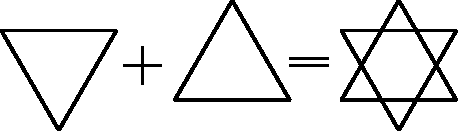
\includegraphics{bartTri.pdf}
\]
But I wanted to know how to draw 5-pointed stars like the other
kids. So one day I taught myself to draw a star like this:
\[
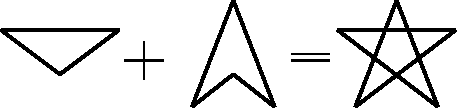
\includegraphics{bartTri2.pdf}
\]
This may seem like a silly way to draw this star---it certainly makes
me chuckle now. Let's see if we can give a theory for drawing stars
that will connect the two different stars above, teach you how to
draw some new stars, and learn a little more mathematics along the
way.

We'll start with $5$ points equally spaced on a circle:
\[
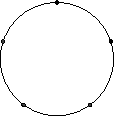
\includegraphics{stfive.pdf}
\]
Think of these points as \textit{pins}.  Next we'll start at the top
and draw lines that we'll think of as \textit{strings}, moving
clockwise to the point two steps away each time:
\[
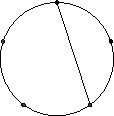
\includegraphics{stfive1.pdf}\qquad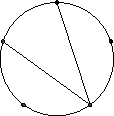
\includegraphics{stfive2.pdf}\qquad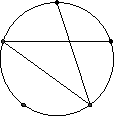
\includegraphics{stfive3.pdf}\qquad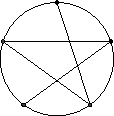
\includegraphics{stfive4.pdf}\qquad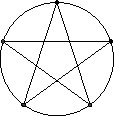
\includegraphics{stfive5.pdf}
\]
Check it out, we got a star! If we had used pins and string to make
this star, we could have done it with one piece of string.

Now start with $6$ points equally spaced on a circle. Again, we'll
move clockwise two steps each time:
\[
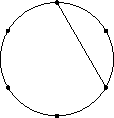
\includegraphics{stsix1.pdf}\qquad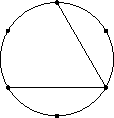
\includegraphics{stsix2.pdf}\qquad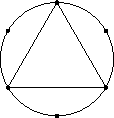
\includegraphics{stsix3.pdf}
\]
Oops, we've run out of points! No worries, just start again at one of
the points that hasn't been touched by a line yet, drawing lines and
moving two steps each time:
\[
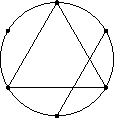
\includegraphics{stsix4.pdf}\qquad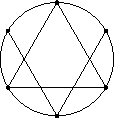
\includegraphics{stsix5.pdf}\qquad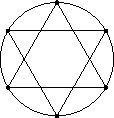
\includegraphics{stsix6.pdf}
\]
Ah! The other star! In this case, if we used pins and strings, we'd
need to use \textit{two} pieces of string. Hmmm---at this point I have
a question:
\begin{question} 
How do we actually draw $n$ equally spaced points on a circle?
\end{question}
 
You can figure that one out---or just ask someone who is standing up at
the front of some room talking to themselves. Oh! And I have another
question:
\begin{question} 
What happens if you put $n$ points, and connect them by moving $s$
steps each time?
\end{question}
I'm feeling generous, so I'll help out with this one. Let's do a bunch
of examples together. I'm hoping that the following notation will help
out:\index{ns@$\star{n}{s}$}
\[
\star{n}{s}=\text{the star with $n$ equally spaced points where we move $s$ steps clockwise}
\]
\begin{warning}
Remember, $\star{n}{s}$ is a star, \textbf{not} a fraction!
\end{warning}
Armed with our new notation, let's draw the following stars!
\[
{
\renewcommand{\arraystretch}{1.5}
\begin{array}{|c|c|c|}\hline
 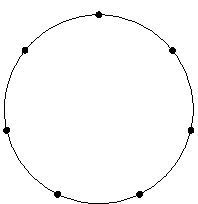
\includegraphics{stseven.pdf} & 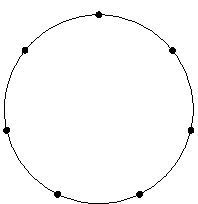
\includegraphics{stseven.pdf} & 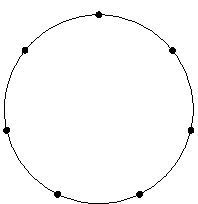
\includegraphics{stseven.pdf} \\
\star{7}{1} & \star{7}{2} & \star{7}{3} \\\hline 
 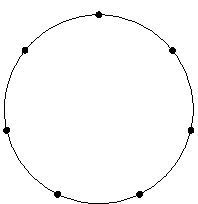
\includegraphics{stseven.pdf} & 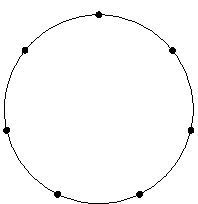
\includegraphics{stseven.pdf} & 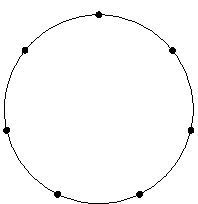
\includegraphics{stseven.pdf} \\
\star{7}{4} & \star{7}{5} & \star{7}{6} \\\hline 
\end{array}
}
\]

\begin{question}
Do you notice any patterns? Why not share your observations with a
friend---or an enemy?
\end{question}


\begin{question}
Looking back, we see that some stars, like $\star{7}{2}$, are one piece (or would use one piece of string). Other stars, like $\star{6}{2}$, are more than one piece. What's the general rule?
\end{question}




\end{document}
